%%%%%%%%%%%%%%%%%%%%%%%%%%%%%%%%%%%%%%%%%%%%%%%%%%%%%%%%%%%%%%%%%%%%%%%%%%%%%%%%%%
\begin{frame}[fragile]\frametitle{}
\begin{center}
{\Large Framework}
\end{center}
\end{frame}

%%%%%%%%%%%%%%%%%%%%%%%%%%%%%%%%%%%%%%%%%%%%%%%%%%%%%%%%%%%
\begin{frame}[fragile]\frametitle{Recap: Retrieval Augmented Generation (RAG)}

\begin{center}
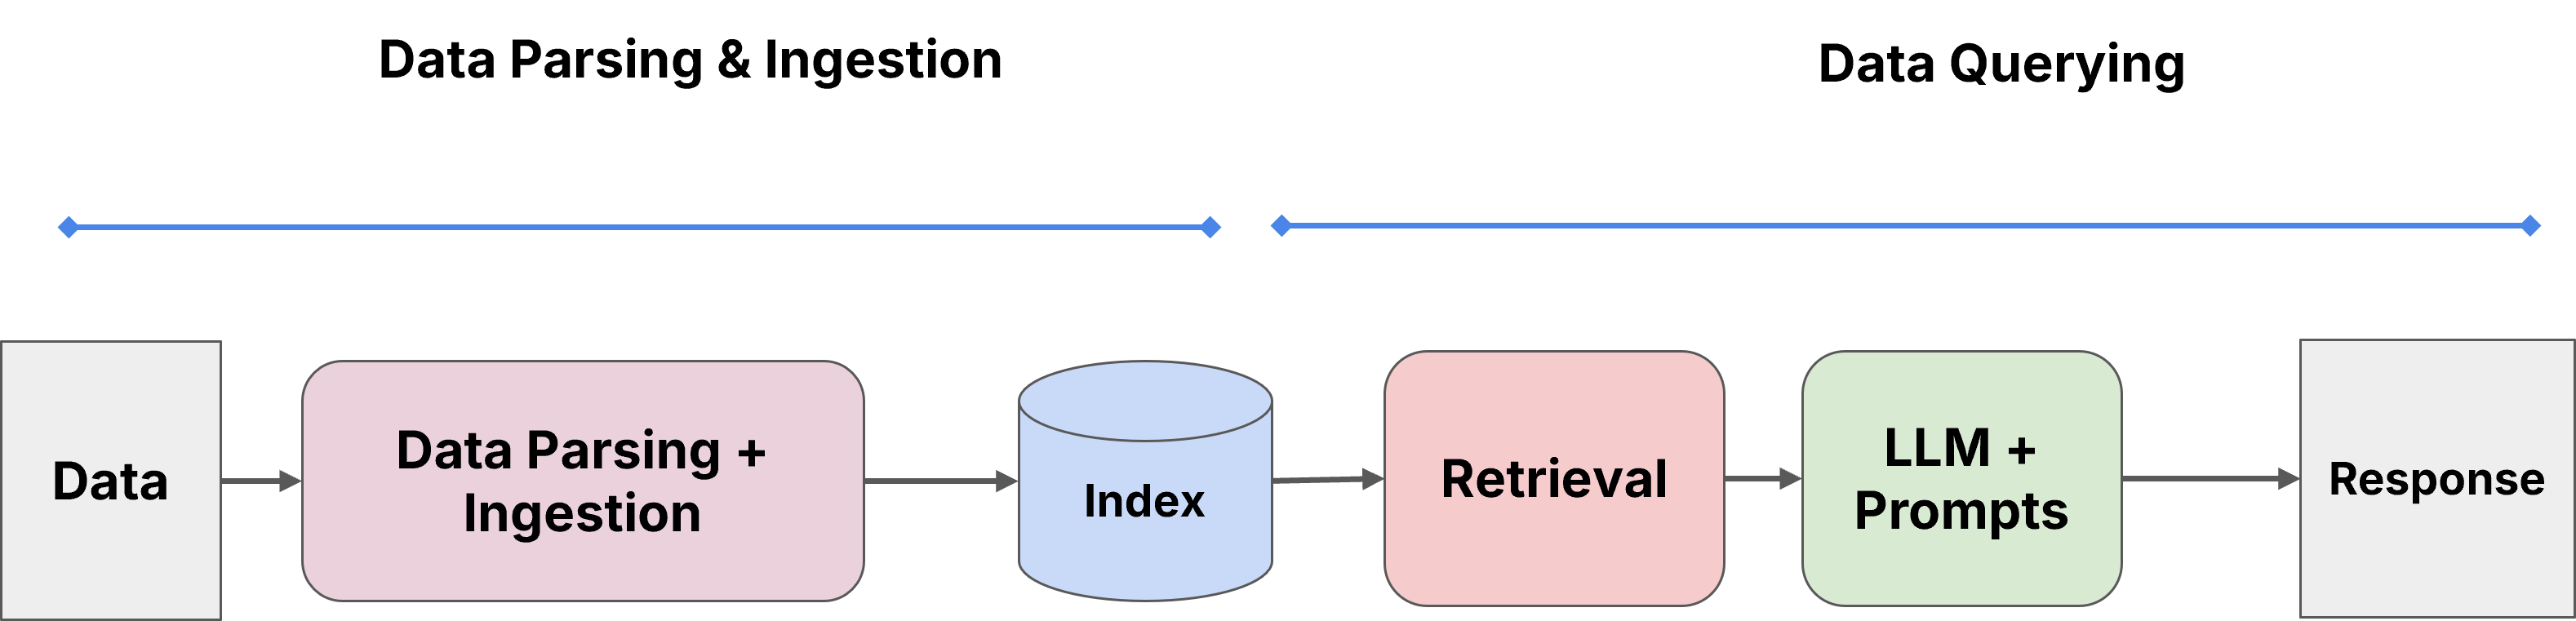
\includegraphics[width=\linewidth,keepaspectratio]{llamaindex1}

{\tiny (Ref: Data AI Summit - Databricks 2024)}
\end{center}
\end{frame}

%%%%%%%%%%%%%%%%%%%%%%%%%%%%%%%%%%%%%%%%%%%%%%%%%%%%%%%%%%%
\begin{frame}[fragile]\frametitle{Recap: Naive RAG}

\begin{center}
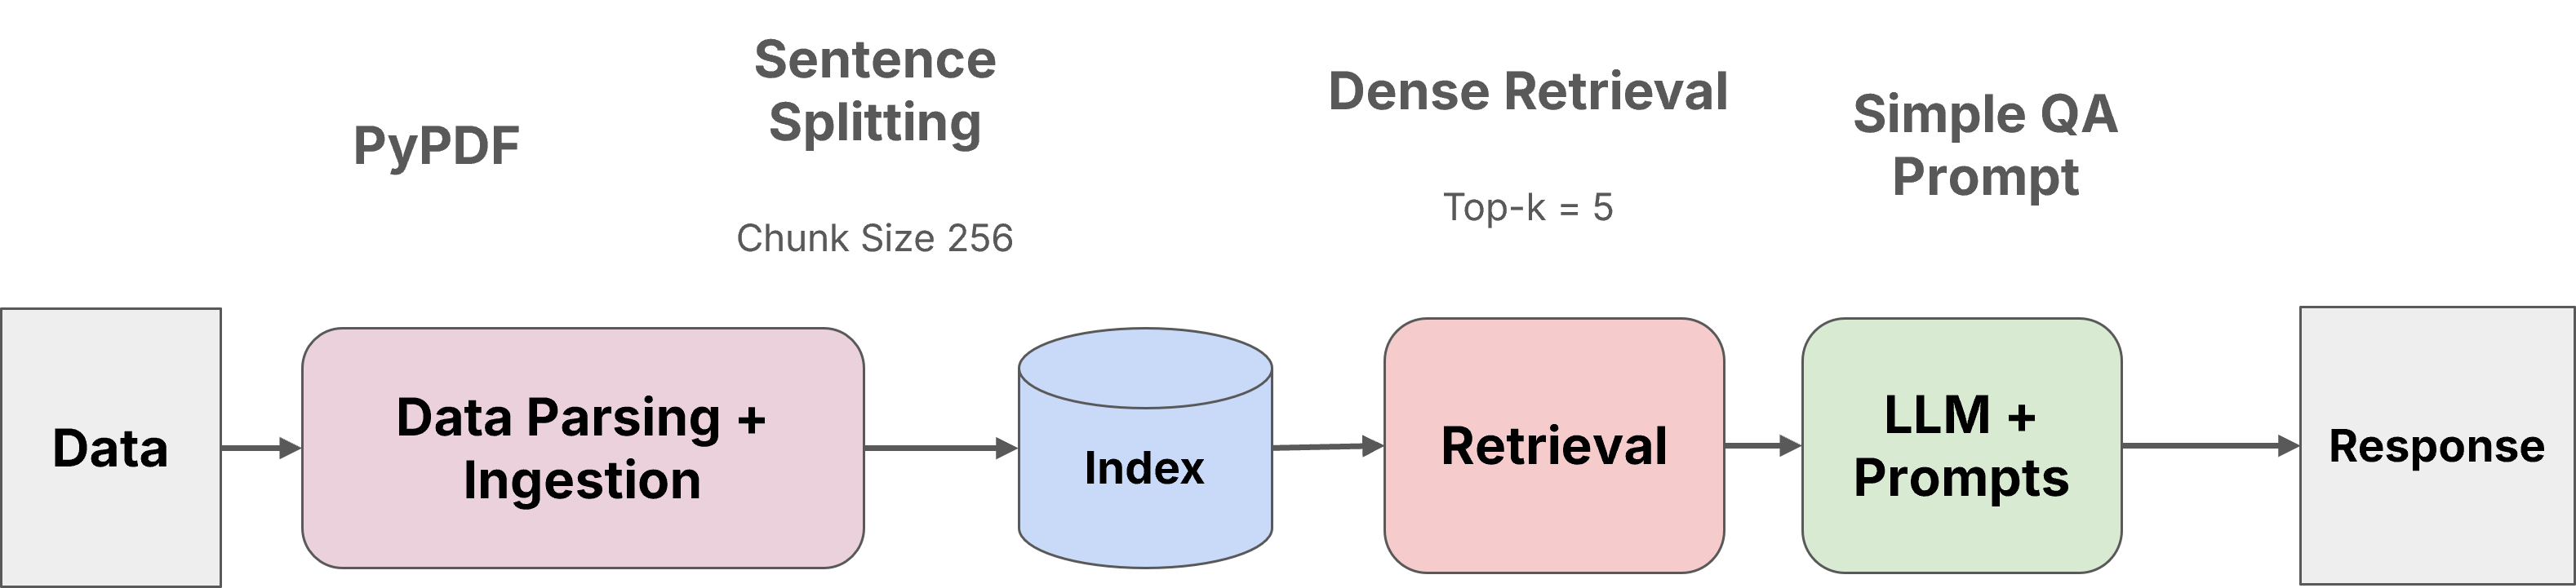
\includegraphics[width=0.8\linewidth,keepaspectratio]{llamaindex2}

{\tiny (Ref: Data AI Summit - Databricks 2024)}
\end{center}
\end{frame}


%%%%%%%%%%%%%%%%%%%%%%%%%%%%%%%%%%%%%%%%%%%%%%%%%%%%%%%%%%%
\begin{frame}[fragile]\frametitle{Challenges with Naive RAG}


\begin{itemize}
\item Easy to Prototype, Hard to Productionize
	\begin{itemize}
	\item Tend to work well for simple questions over a simple, small set of documents
	\item But productionizing RAG over more questions and a larger set of data is hard!
	\end{itemize}	
\item Failure Modes:
	\begin{itemize}
	\item Simple Questions over Complex Data
	\item Simple Questions over Multiple Documents
	\item Complex Questions 
	\end{itemize}	
\item In the naive setting, RAG is boring
	\begin{itemize}
	\item It's just a glorified search system
	\item There's many questions/tasks that naive RAG can’t give an answer to
	\item Can we build a general context-augmented research assistant?
	\end{itemize}		
\end{itemize}	

{\tiny (Ref: Data AI Summit - Databricks 2024)}

\end{frame}

%%%%%%%%%%%%%%%%%%%%%%%%%%%%%%%%%%%%%%%%%%%%%%%%%%%%%%%%%%%
\begin{frame}[fragile]\frametitle{Main Focus Areas}

\begin{center}
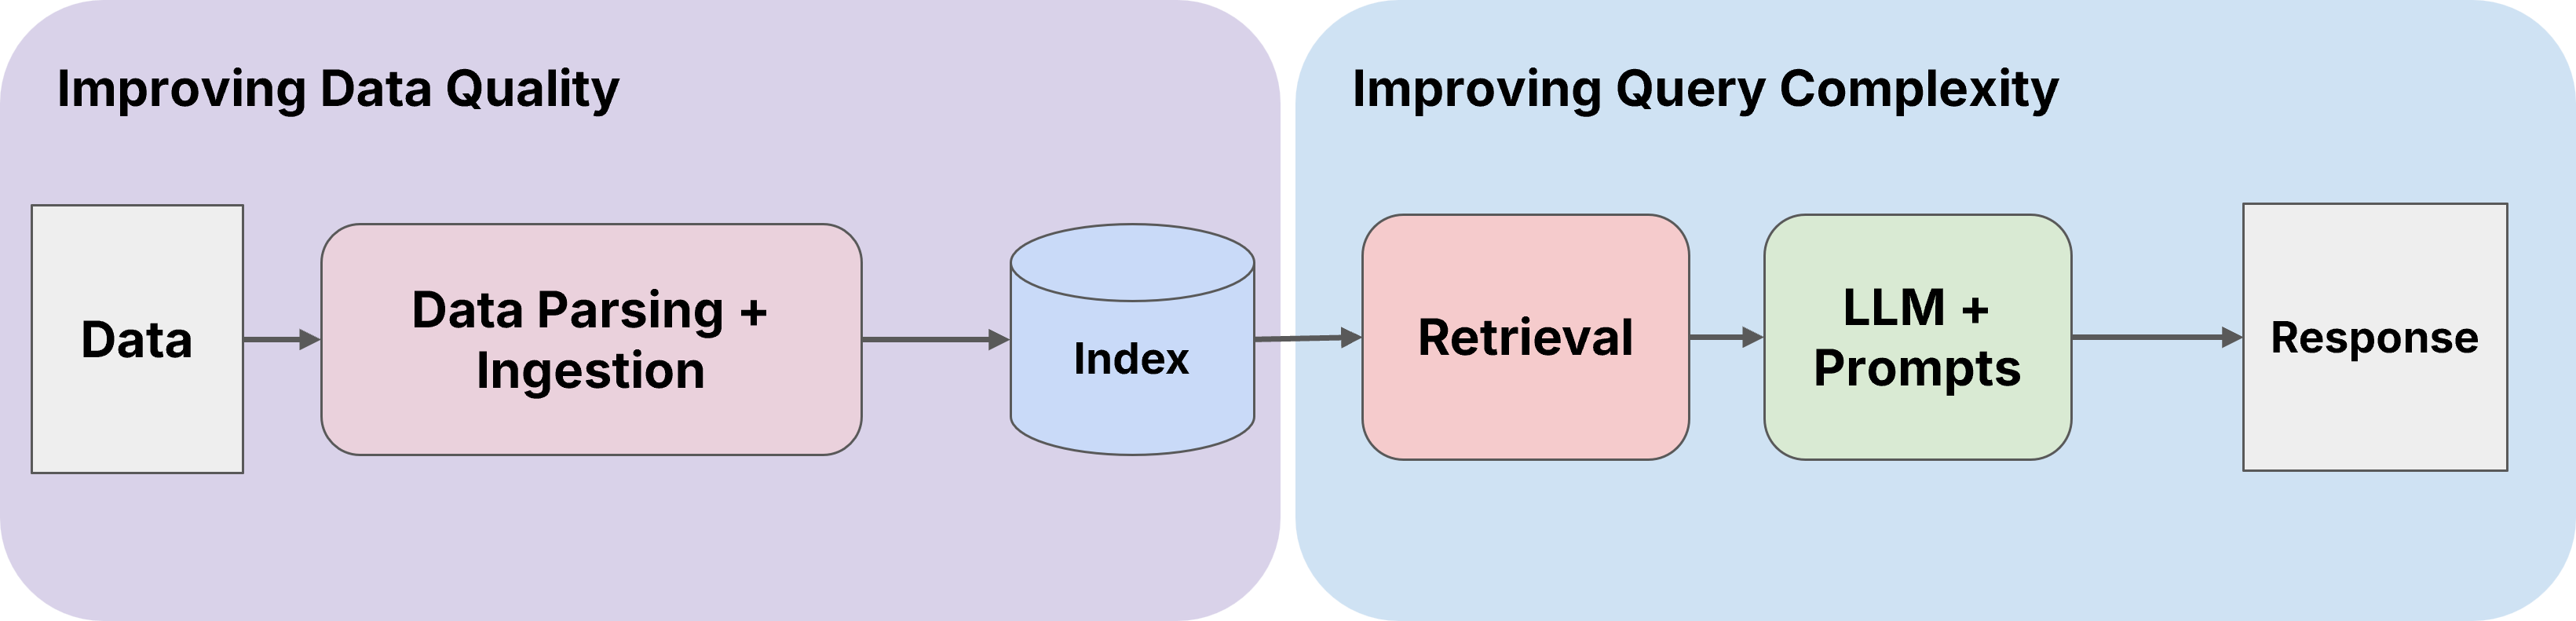
\includegraphics[width=\linewidth,keepaspectratio]{llamaindex3}

{\tiny (Ref: Data AI Summit - Databricks 2024)}
\end{center}
\end{frame}

%%%%%%%%%%%%%%%%%%%%%%%%%%%%%%%%%%%%%%%%%%%%%%%%%%%%%%%%%%%%%%%%%%%%%%%%%%%%%%%%%%
\begin{frame}[fragile]\frametitle{}
\begin{center}
{\Large Improving Data Quality}
\end{center}
\end{frame}

%%%%%%%%%%%%%%%%%%%%%%%%%%%%%%%%%%%%%%%%%%%%%%%%%%%%%%%%%%%
\begin{frame}[fragile]\frametitle{RAG is only as Good as your Data}

Garbage in $=$ Garbage Out

\begin{center}
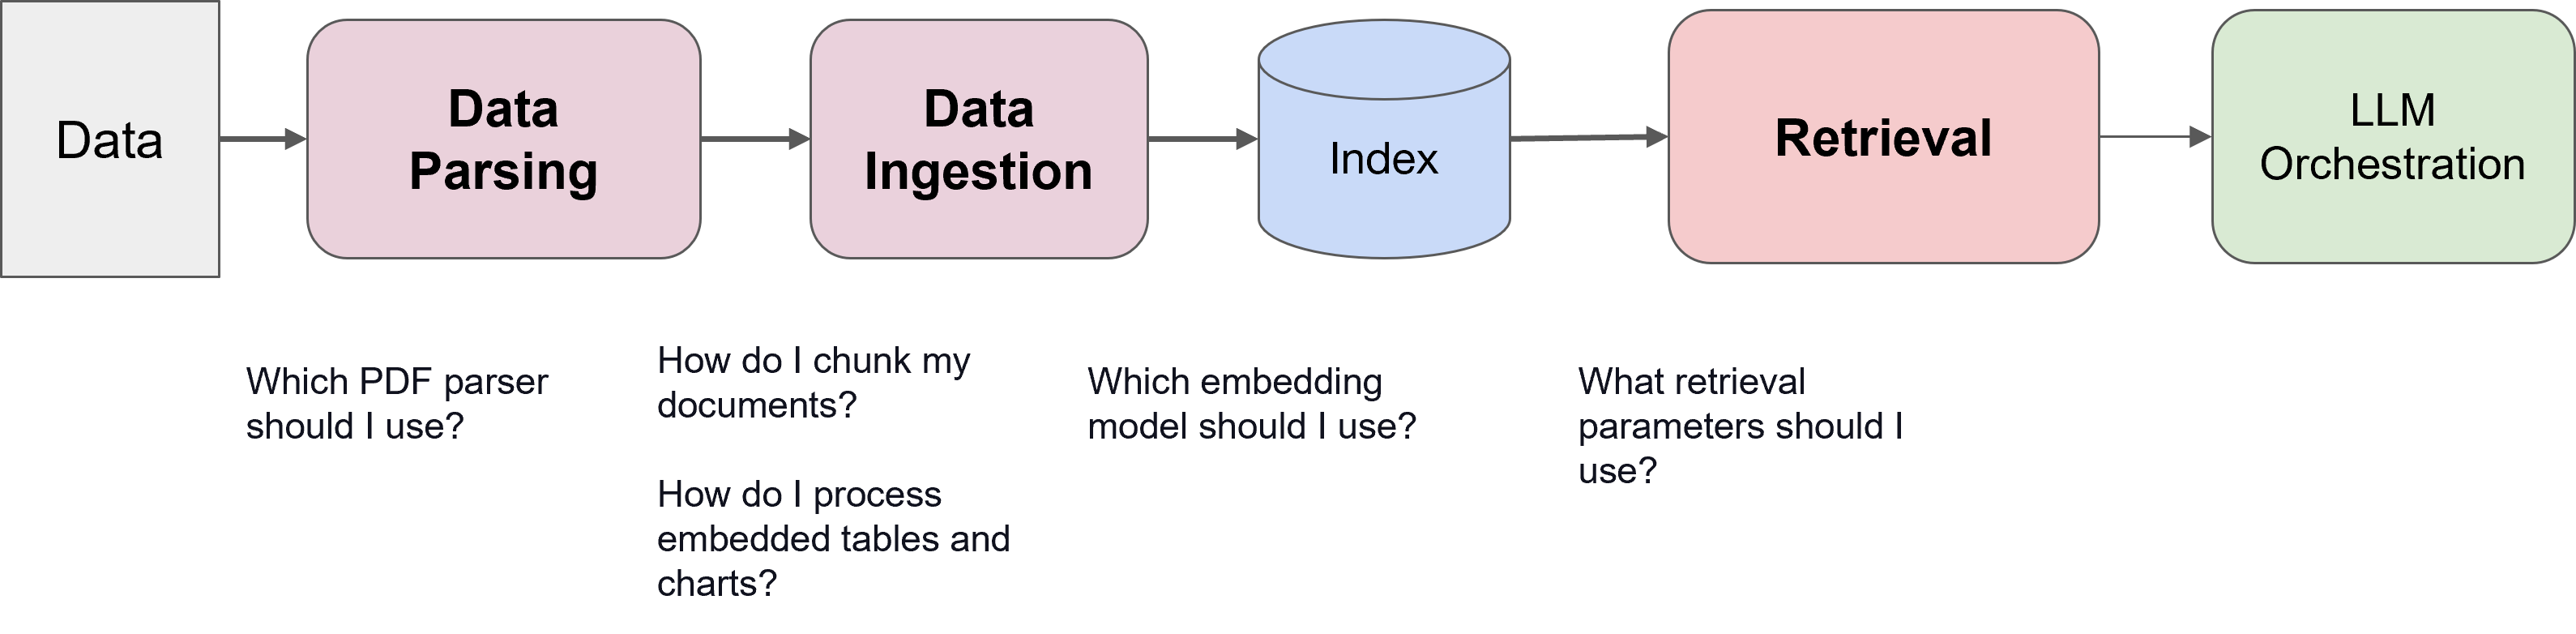
\includegraphics[width=\linewidth,keepaspectratio]{llamaindex4}

{\tiny (Ref: Data AI Summit - Databricks 2024)}
\end{center}
\end{frame}


%%%%%%%%%%%%%%%%%%%%%%%%%%%%%%%%%%%%%%%%%%%%%%%%%%%%%%%%%%%
\begin{frame}[fragile]\frametitle{RAG is only as Good as your Data}


\begin{center}
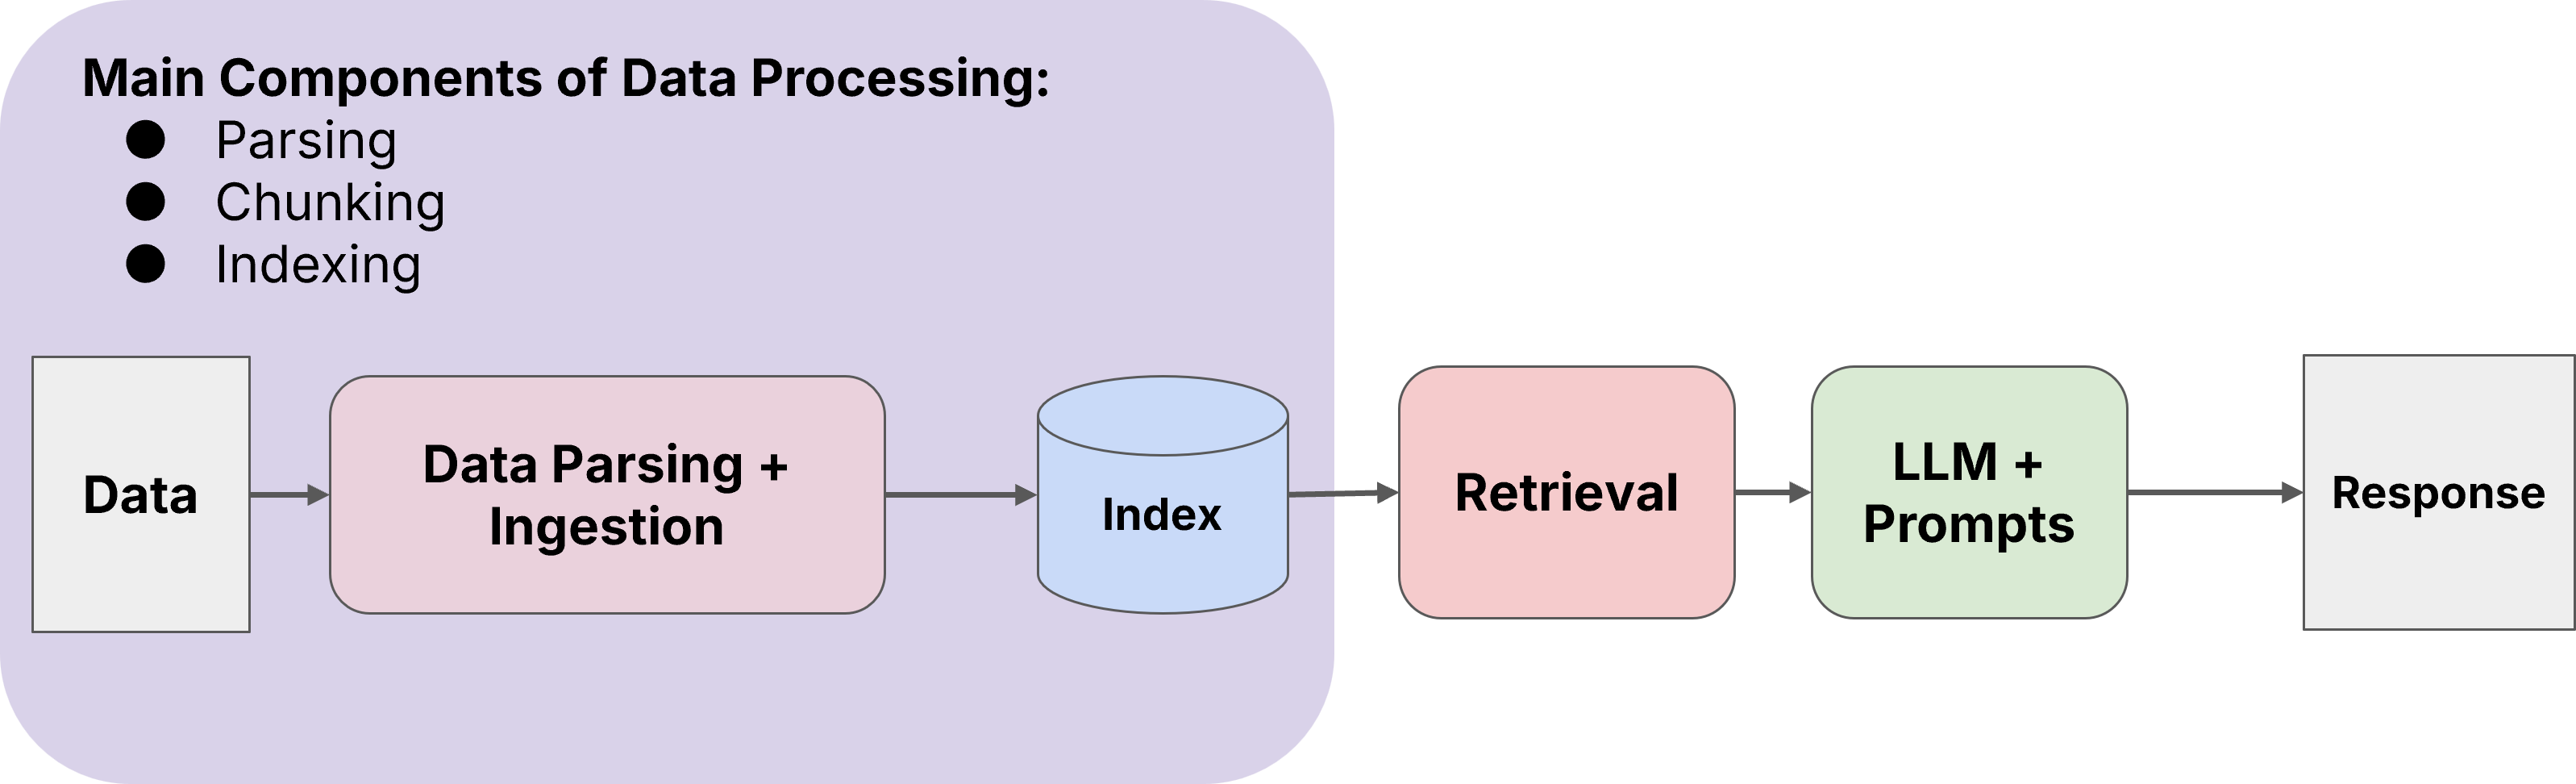
\includegraphics[width=\linewidth,keepaspectratio]{llamaindex5}

{\tiny (Ref: Data AI Summit - Databricks 2024)}
\end{center}
\end{frame}


%%%%%%%%%%%%%%%%%%%%%%%%%%%%%%%%%%%%%%%%%%%%%%%%%%%%%%%%%%%
\begin{frame}[fragile]\frametitle{General Principles}


\begin{itemize}
\item Parsing:
	\begin{itemize}
	\item Bad parsers are a key cause of garbage in == garbage out.
	\item Badly formatted text/tables confuse even the best LLMs
	\end{itemize}	
\item Chunking: 
	\begin{itemize}
	\item Try to preserve semantically similar content, say, 5 Levels of Text Splitting
	\item Strong baseline: page-level chunking
	\end{itemize}	
\item Indexing:
	\begin{itemize}
	\item Raw text often times confuses the embedding model
	\item Don’t just embed the raw text, embed references
	\item Having multiple embeddings point to the same chunk is a good practice! 
	\end{itemize}		
\end{itemize}	

{\tiny (Ref: Data AI Summit - Databricks 2024)}

\end{frame}

%%%%%%%%%%%%%%%%%%%%%%%%%%%%%%%%%%%%%%%%%%%%%%%%%%%%%%%%%%%
\begin{frame}[fragile]\frametitle{Case Study: Complex Documents}

\begin{columns}
    \begin{column}[T]{0.4\linewidth}
	A lot of documents can be classified as complex: 

		\begin{itemize}
		\item Embedded Tables, Charts, Images
		\item Irregular Layouts
		\item Headers/Footers
		\end{itemize}	
Naive RAG indexing pipelines fail over these documents.
		
    \end{column}
    \begin{column}[T]{0.6\linewidth}
		\begin{center}
		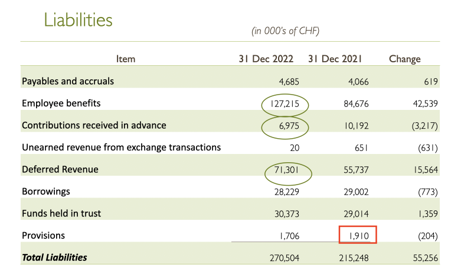
\includegraphics[width=\linewidth,keepaspectratio]{llamaindex6}

		{\tiny (Ref: Data AI Summit - Databricks 2024)}  
		\end{center}
    \end{column}
  \end{columns}
  
\end{frame}

%%%%%%%%%%%%%%%%%%%%%%%%%%%%%%%%%%%%%%%%%%%%%%%%%%%%%%%%%%%
\begin{frame}[fragile]\frametitle{Most PDF Parsing is Inadequate}
Extracts into a messy format that is impossible to pass down into more advanced ingestion/retrieval algorithms.


\begin{center}
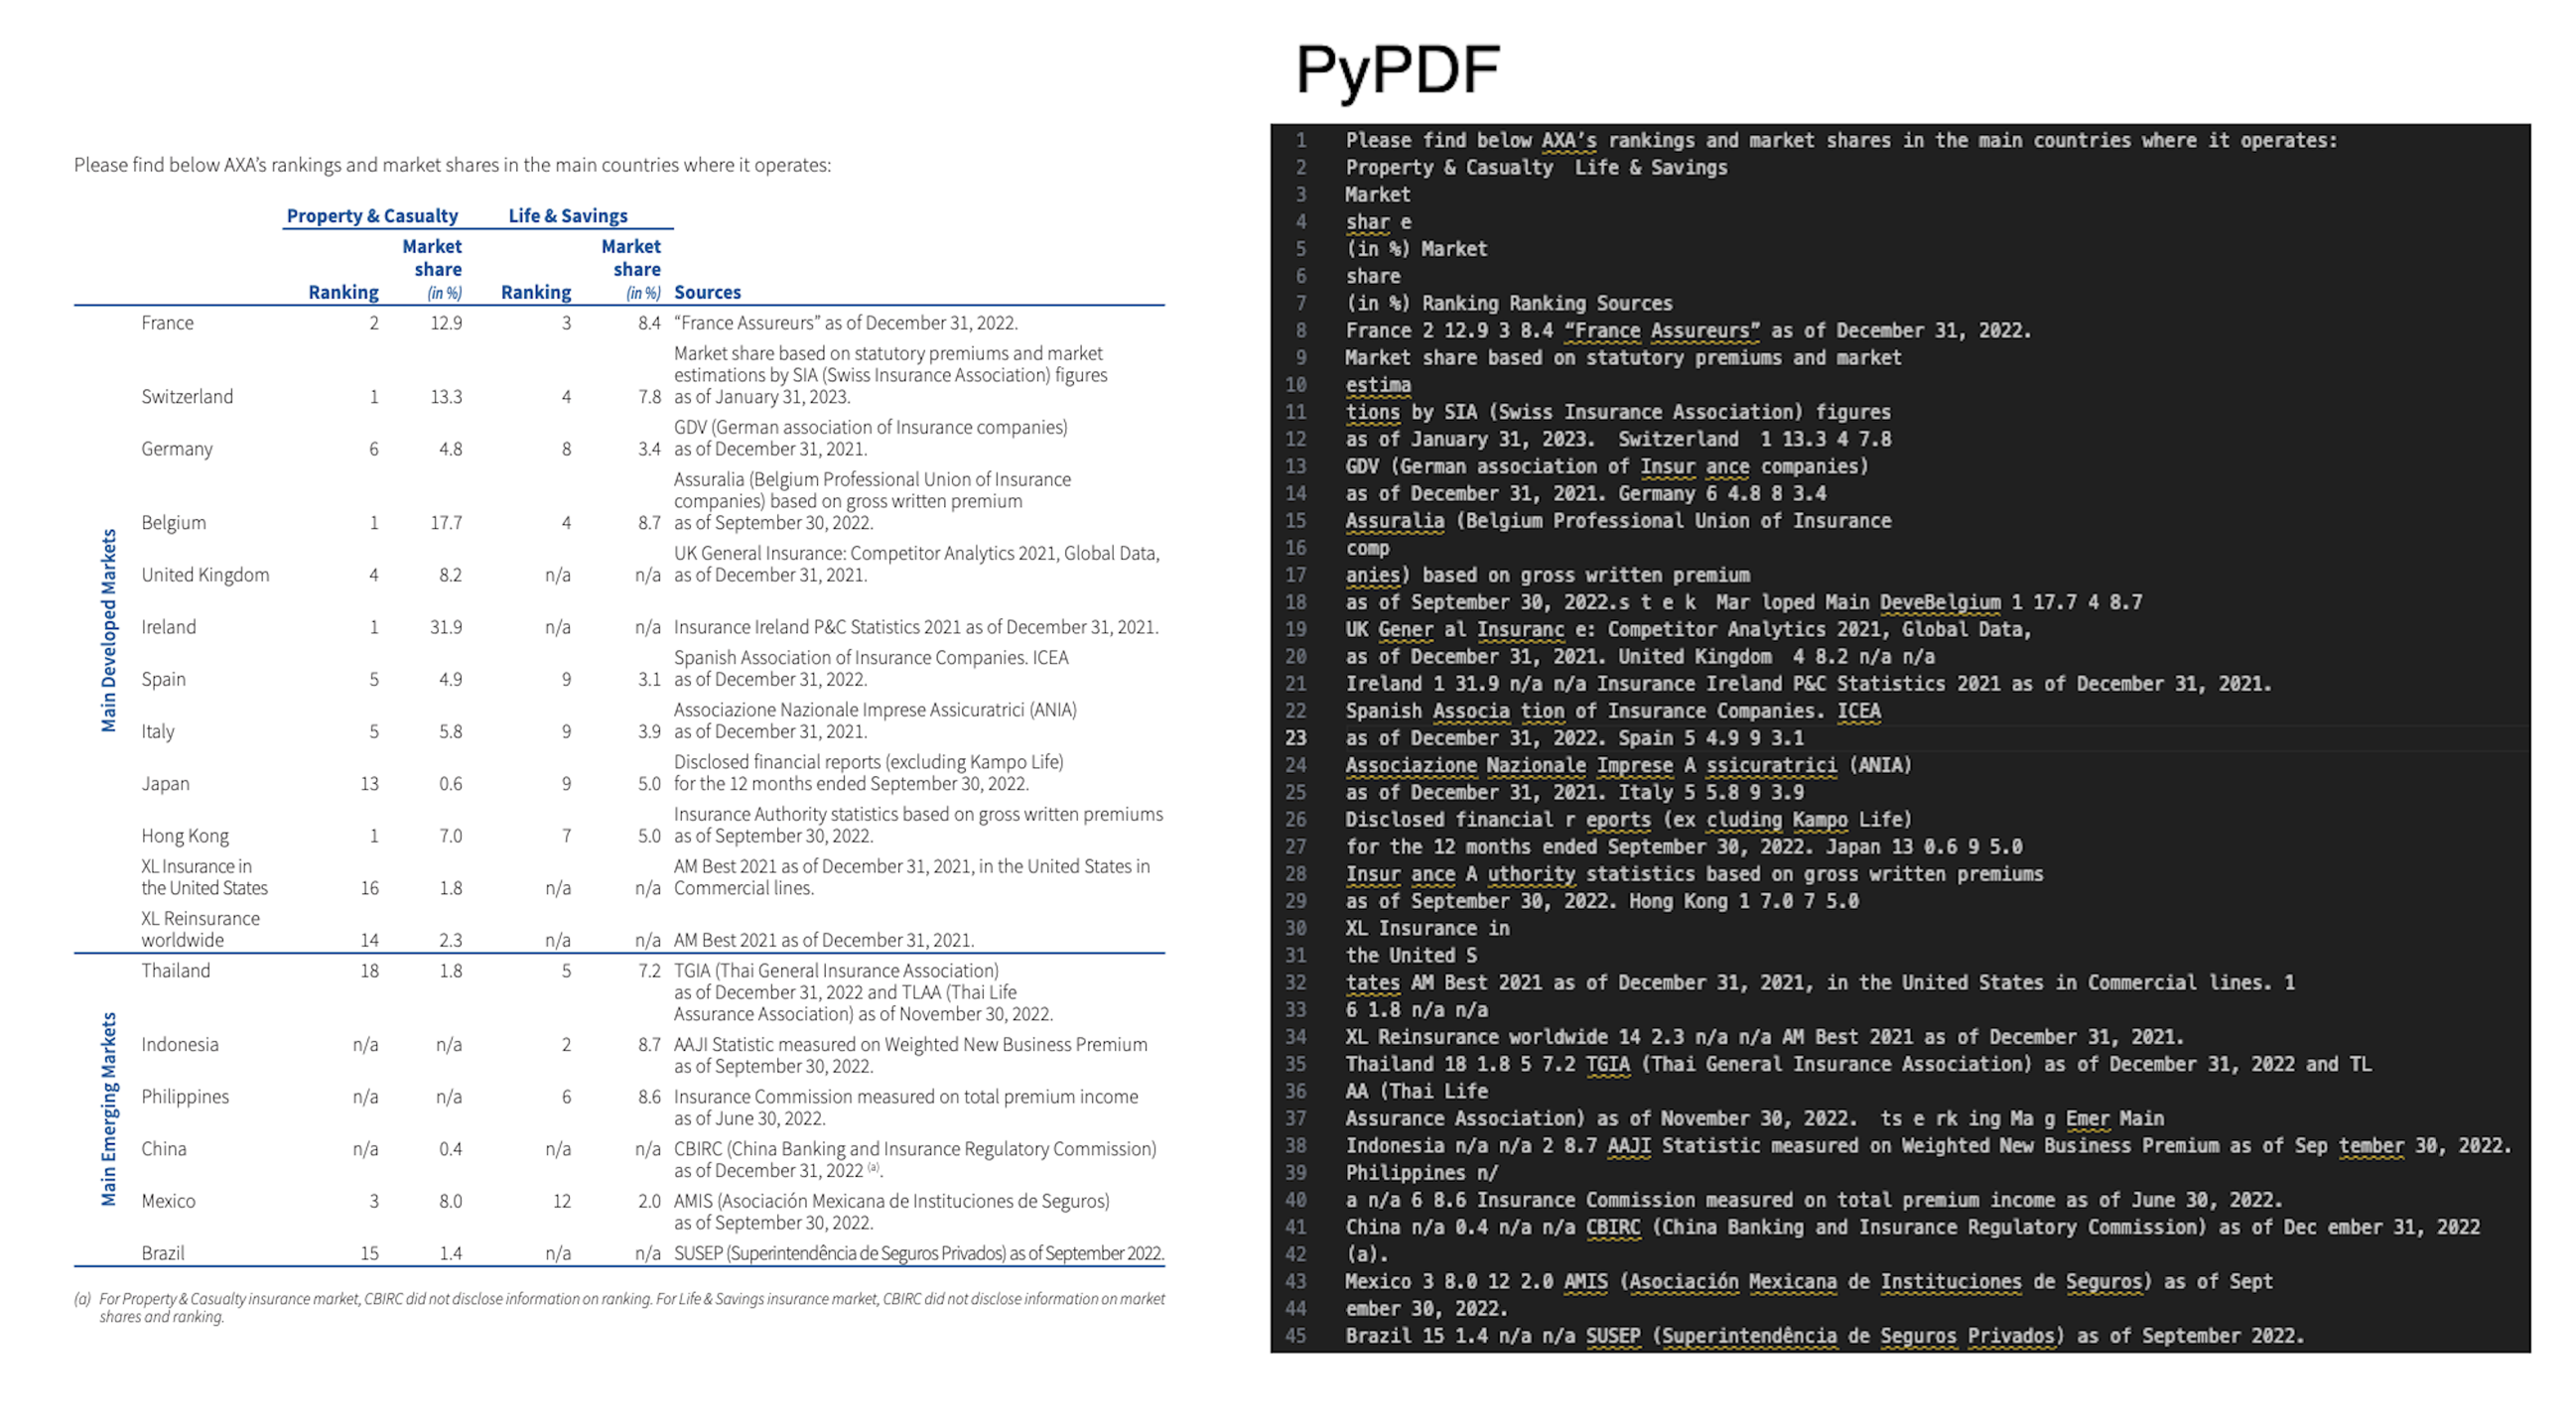
\includegraphics[width=\linewidth,keepaspectratio]{llamaindex7}

{\tiny (Ref: Data AI Summit - Databricks 2024)}
\end{center}
\end{frame}

%%%%%%%%%%%%%%%%%%%%%%%%%%%%%%%%%%%%%%%%%%%%%%%%%%%%%%%%%%%
\begin{frame}[fragile]\frametitle{LlamaParse}
A special Document Parser designed to let you build RAG over Complex docs
https://github.com/run-llama/llama\_parse


\begin{columns}
    \begin{column}[T]{0.4\linewidth}
Capabilities:
		\begin{itemize}
		\item Extracts tables / charts
		\item Input natural language parsing instructions
		\item JSON mode
		\item Image Extraction
		\item Support for more than 10 document types (.pdf, .pptx, .docx, .xml)

		\end{itemize}	
		
    \end{column}
    \begin{column}[T]{0.6\linewidth}
		\begin{center}
		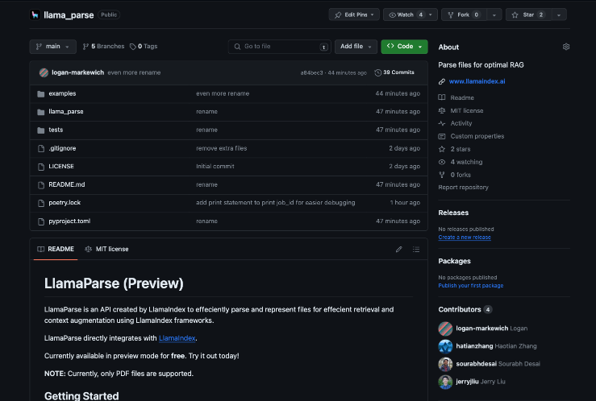
\includegraphics[width=0.8\linewidth,keepaspectratio]{llamaindex8}

		{\tiny (Ref: Data AI Summit - Databricks 2024)}
		\end{center}
    \end{column}
  \end{columns}
  
\end{frame}

%%%%%%%%%%%%%%%%%%%%%%%%%%%%%%%%%%%%%%%%%%%%%%%%%%%%%%%%%%%
\begin{frame}[fragile]\frametitle{LlamaParse $+$ Advanced Indexing}


\begin{columns}
    \begin{column}[T]{0.4\linewidth}

		\begin{itemize}
		\item Use LlamaParse to parse a document into a semi-structured markdown representation (text + tables)
		\item Use a markdown parser to extract out text and table chunks
		\item Use an LLM to extract a summary from each table → link to underlying table chunk.
		\item Index a graph of text and table chunks.
		\end{itemize}	
		
    \end{column}
    \begin{column}[T]{0.6\linewidth}
		\begin{center}
		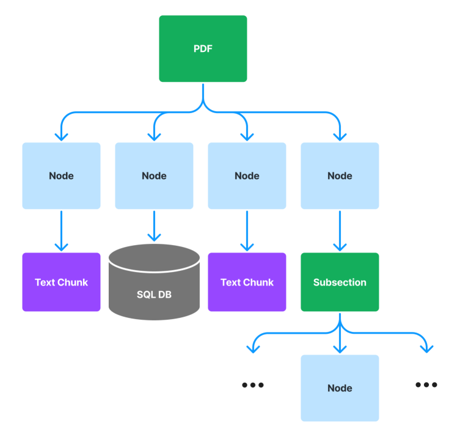
\includegraphics[width=0.8\linewidth,keepaspectratio]{llamaindex9}

		{\tiny (Ref: Data AI Summit - Databricks 2024)}
		\end{center}
    \end{column}
  \end{columns}
  


\end{frame}



%%%%%%%%%%%%%%%%%%%%%%%%%%%%%%%%%%%%%%%%%%%%%%%%%%%%%%%%%%%%%%%%%%%%%%%%%%%%%%%%%%
\begin{frame}[fragile]\frametitle{}
\begin{center}
{\Large Improving Query Complexity}
\end{center}
\end{frame}


%%%%%%%%%%%%%%%%%%%%%%%%%%%%%%%%%%%%%%%%%%%%%%%%%%%%%%%%%%%
\begin{frame}[fragile]\frametitle{Complex Questions}
There's certain questions we want to ask where naive RAG will fail.

Examples:
\begin{itemize}
\item Summarization Questions: ``Give me a summary of the entire annual report''
\item Comparison Questions: ``Compare the open-source contributions of candidate A and candidate B.''
\item Structured Analytics $+$ Semantic Search: ``Tell me about the risk factors of the highest-performing ride-share company in the US''
\item General Multi-part Questions: ``Tell me about the pro-X arguments in article A, and tell me about the pro-Y arguments in article B, make a table based on our internal style guide, then generate your own conclusion based on these facts.''
\end{itemize}	
		

 		{\tiny (Ref: Data AI Summit - Databricks 2024)}

\end{frame}

%%%%%%%%%%%%%%%%%%%%%%%%%%%%%%%%%%%%%%%%%%%%%%%%%%%%%%%%%%%
\begin{frame}[fragile]\frametitle{Query Planning}

\begin{itemize}
\item Break down query into parallelizable sub-queries.
\item Each can be execute-query-ed against any set of RAG pipelines
\item Example: Compare revenue of Uber and Lyft in 2021
\end{itemize}	

\begin{center}
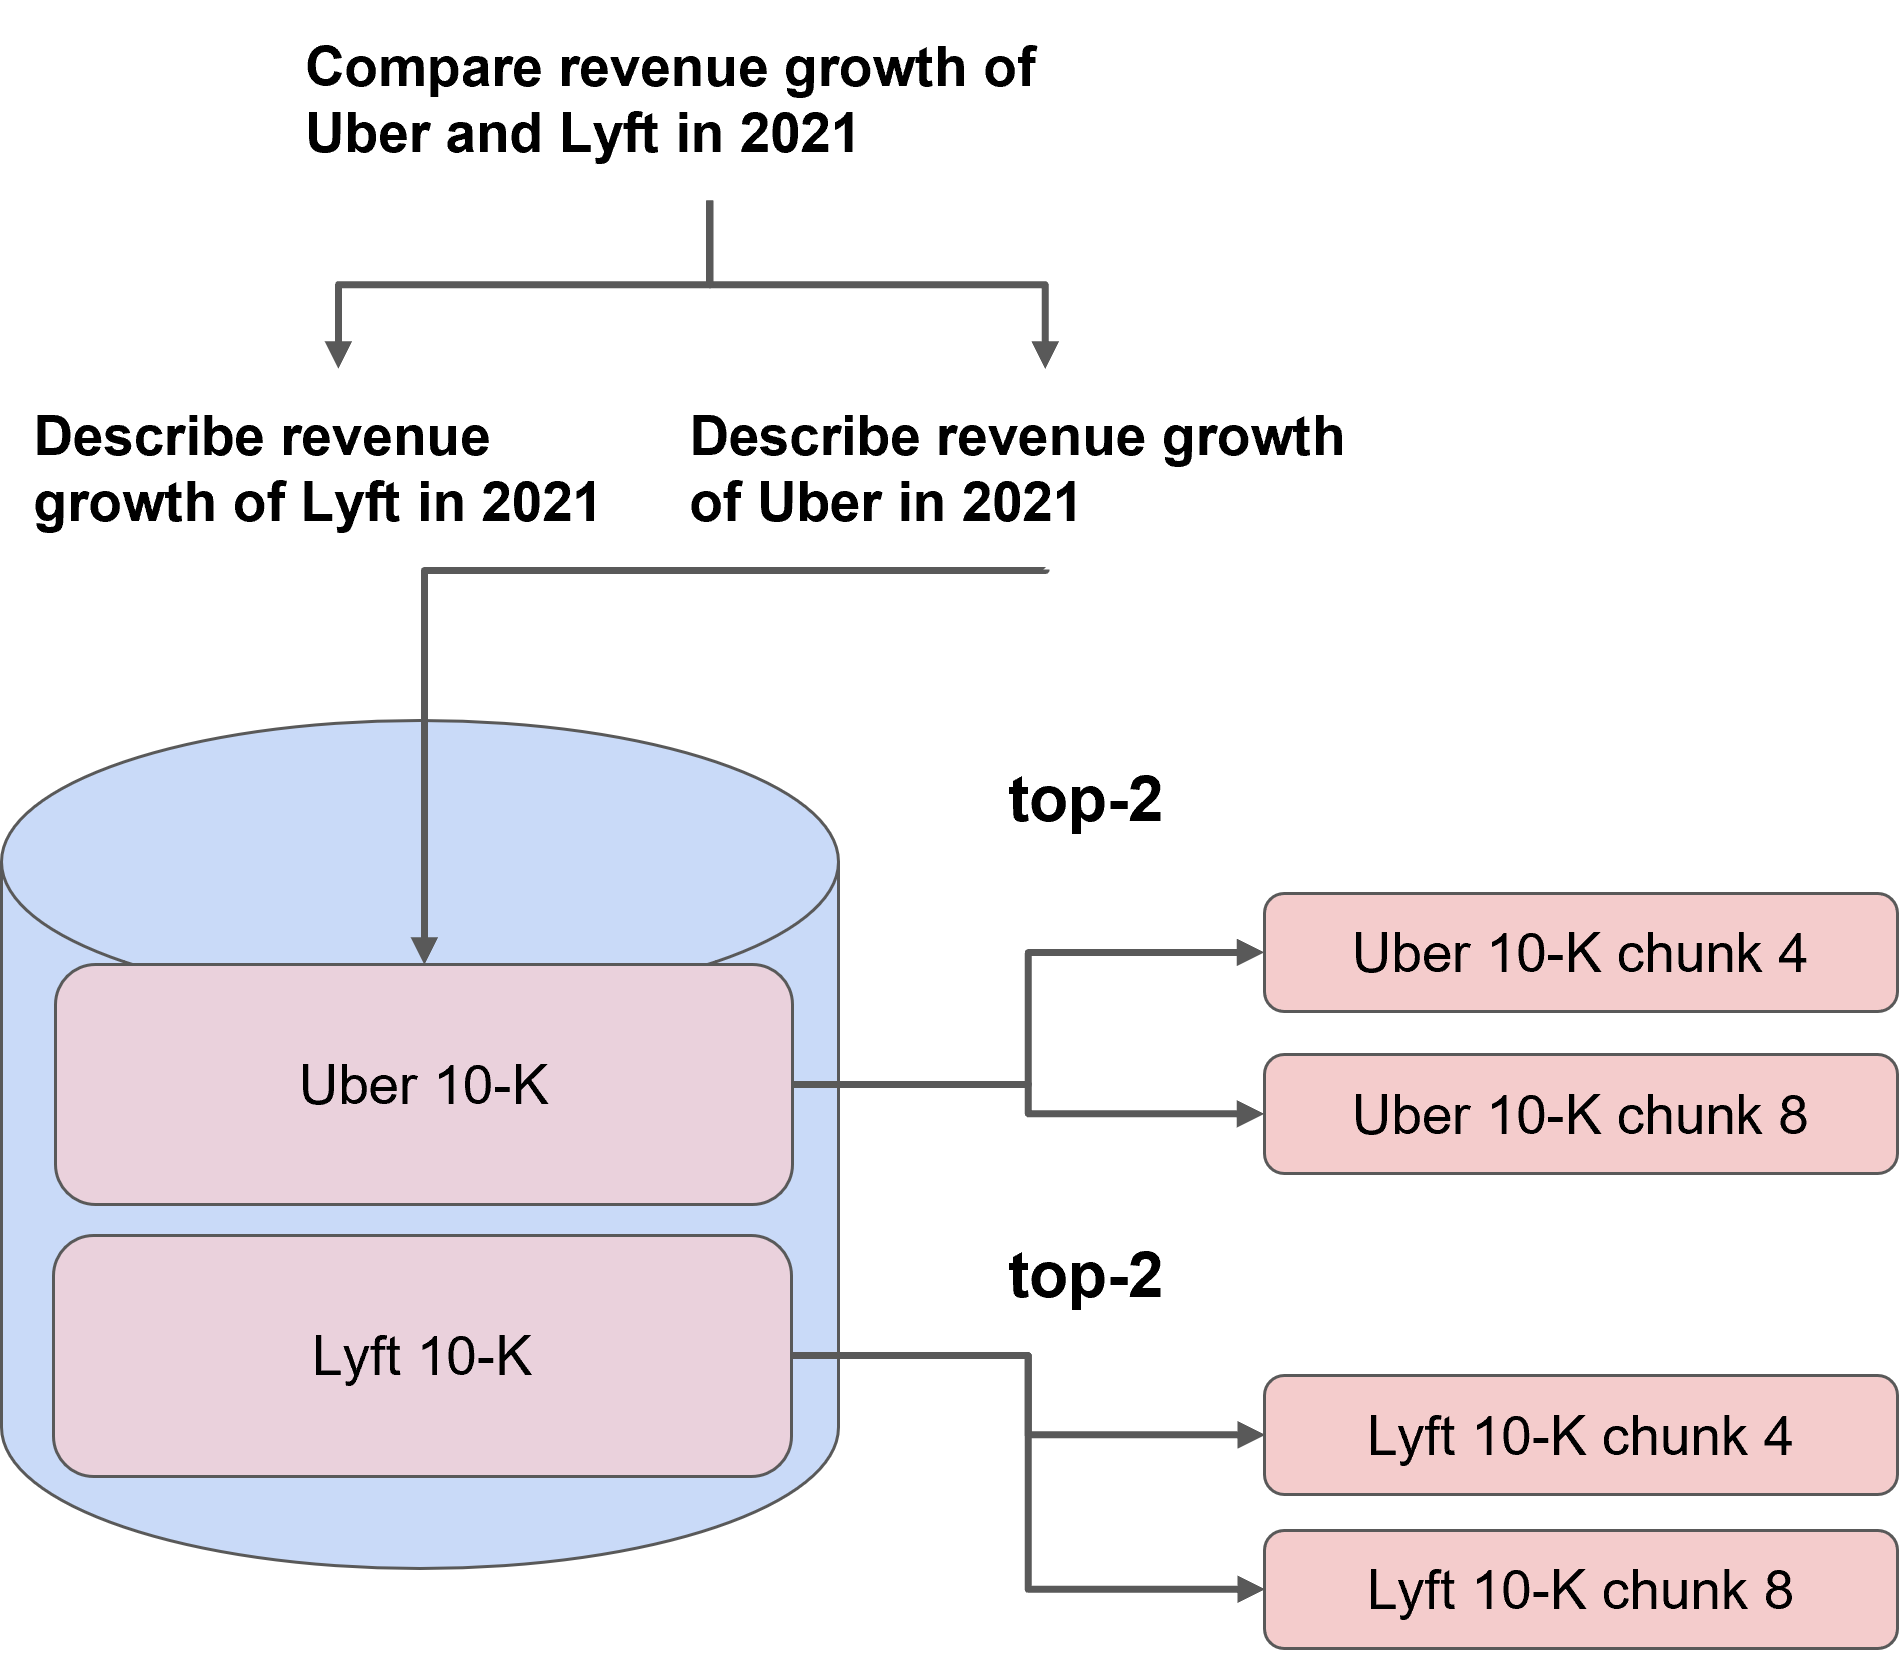
\includegraphics[width=0.5\linewidth,keepaspectratio]{llamaindex10}

{\tiny (Ref: Data AI Summit - Databricks 2024)}
\end{center}
\end{frame}

% %%%%%%%%%%%%%%%%%%%%%%%%%%%%%%%%%%%%%%%%%%%%%%%%%%%%%%%%%%%
% \begin{frame}[fragile]\frametitle{Tool Use}

% \begin{columns}
    % \begin{column}[T]{0.4\linewidth}

		% \begin{itemize}
		% \item Use an LLM to call an API
		% \item Infer the parameters of that API
		% \item In normal RAG you just pass through the query.
		% \item But what if you used the LLM to infer all the parameters for the API interface?
		% \item A key capability in many QA use cases (auto-retrieval, text-to-SQL, and more)
		% \end{itemize}	
		
    % \end{column}
    % \begin{column}[T]{0.6\linewidth}
		% \begin{center}
		% 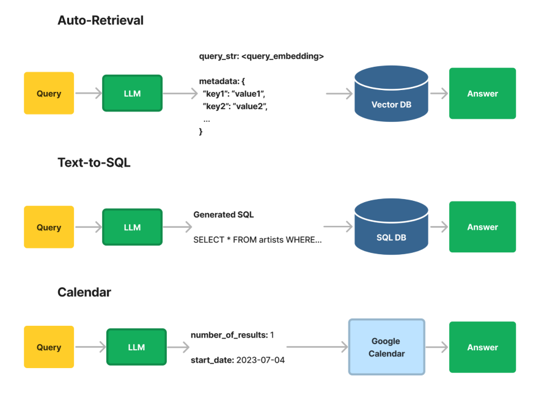
\includegraphics[width=0.8\linewidth,keepaspectratio]{llamaindex11}

		% {\tiny (Ref: Data AI Summit - Databricks 2024)}
		% \end{center}
    % \end{column}
  % \end{columns}

% \end{frame}

%%%%%%%%%%%%%%%%%%%%%%%%%%%%%%%%%%%%%%%%%%%%%%%%%%%%%%%%%%%%%%%%%%%%%%%%%%%%%%%%%%
\begin{frame}[fragile]\frametitle{}
\begin{center}
{\Large Concepts}
\end{center}
\end{frame}



%%%%%%%%%%%%%%%%%%%%%%%%%%%%%%%%%%%%%%%%%%%%%%%%%%%%%%%%%%%
\begin{frame}[fragile]\frametitle{Work-flow}

\begin{center}
\includegraphics[width=\linewidth,keepaspectratio]{llm18}

{\tiny (Ref: LlamaIndex: A Central Interface between LLM's + your external data)}
\end{center}
\end{frame}



%%%%%%%%%%%%%%%%%%%%%%%%%%%%%%%%%%%%%%%%%%%%%%%%%%%%%%%%%%%
\begin{frame}[fragile]\frametitle{Data Connectors: powered by LlamaHub}


\begin{itemize}
\item Easily ingest any kind of data, from anywhere, into unified document containers 
\item Powered by community-driven hub, rapidly growing (90+ loaders and counting!)
\item Growing support for multimodal documents (e.g. with inline images)
\end{itemize}	

$<10$ lines of code to ingest from Notion

\begin{center}
\includegraphics[width=0.8\linewidth,keepaspectratio]{llm16}

{\tiny (Ref: LlamaIndex: A Central Interface between LLM's + your external data)}
\end{center}
\end{frame}

%%%%%%%%%%%%%%%%%%%%%%%%%%%%%%%%%%%%%%%%%%%%%%%%%%%%%%%%%%%
\begin{frame}[fragile]\frametitle{Data Indices + Query Interface}


\begin{itemize}
\item Source documents are stored in a data collection, In-memory, MongoDB
\item Data indices help to provide a view of your raw data, Vectors, keyword lookups, summaries
\item A retriever helps to retrieve relevant documents for your query
\item A query engine manages retrieval and synthesis given the query. 
\end{itemize}	

\begin{center}
\includegraphics[width=0.6\linewidth,keepaspectratio]{llm17}

{\tiny (Ref: LlamaIndex: A Central Interface between LLM's + your external data)}
\end{center}

\end{frame}

%%%%%%%%%%%%%%%%%%%%%%%%%%%%%%%%%%%%%%%%%%%%%%%%%%%%%%%%%%%
\begin{frame}[fragile]\frametitle{Data Ingestion: LlamaHub}


\begin{center}
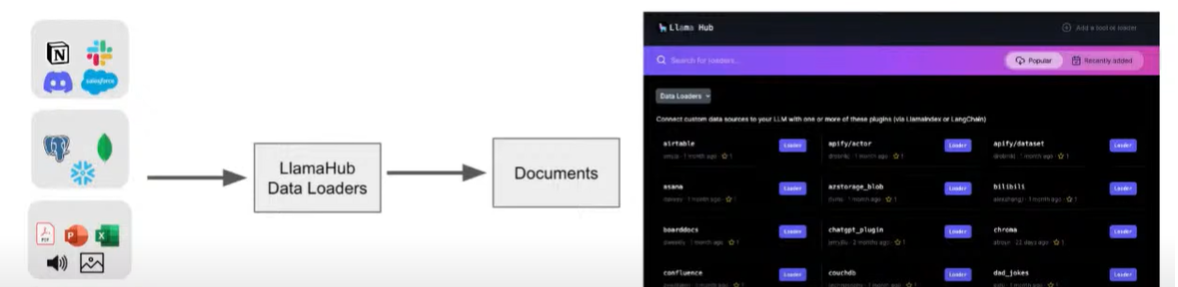
\includegraphics[width=\linewidth,keepaspectratio]{llamaindex12}

{\tiny (Ref: Getting started with LlamaIndex - AI Planet)}
\end{center}
\end{frame}


%%%%%%%%%%%%%%%%%%%%%%%%%%%%%%%%%%%%%%%%%%%%%%%%%%%%%%%%%%%
\begin{frame}[fragile]\frametitle{Data Indexing}

\begin{itemize}
\item Documents are split ie chunking and embedding for each chunk is created
\item Chunk $+$ Embedding is capsuled as 'Node'.
\item All Nodes are stored in 'in-memory index' or Vector Db (e.g. PineCone, Weaviate, Qdrant)
\end{itemize}	

\begin{center}
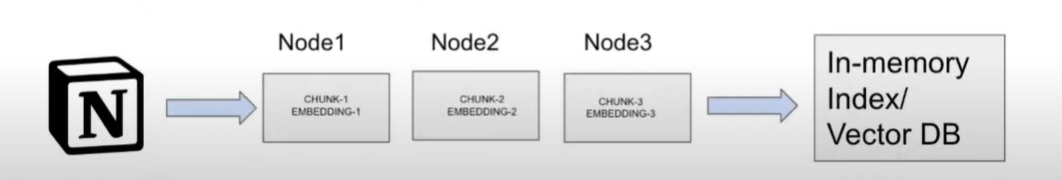
\includegraphics[width=\linewidth,keepaspectratio]{llamaindex13}

{\tiny (Ref: Getting started with LlamaIndex - AI Planet)}
\end{center}
\end{frame}



%%%%%%%%%%%%%%%%%%%%%%%%%%%%%%%%%%%%%%%%%%%%%%%%%%%%%%%%%%%
\begin{frame}[fragile]\frametitle{Vector Store Index}

Nodes are stored in Vector Db, where each node has chunk $+$ embedding.

\begin{center}
\includegraphics[width=0.8\linewidth,keepaspectratio]{llm19}

{\tiny (Ref: LlamaIndex: A Central Interface between LLM's + your external data)}
\end{center}
\end{frame}

%%%%%%%%%%%%%%%%%%%%%%%%%%%%%%%%%%%%%%%%%%%%%%%%%%%%%%%%%%%
\begin{frame}[fragile]\frametitle{Retrieval}

When User asks a query:
\begin{itemize}
\item It retrieves the relevant nodes, ranks them based on the embedding similarity between query and nodes.
\item Post processes the retrieved nodes if needed.
\item Directs the processed nodes to Response Synthesis module.
\end{itemize}	



\begin{center}
\includegraphics[width=0.6\linewidth,keepaspectratio]{llm20}

{\tiny (Ref: LlamaIndex: A Central Interface between LLM's + your external data)}
\end{center}
\end{frame}

%%%%%%%%%%%%%%%%%%%%%%%%%%%%%%%%%%%%%%%%%%%%%%%%%%%%%%%%%%%
\begin{frame}[fragile]\frametitle{Response Synthesis}

Collect answers from all, then collate and then send to final answer.

\begin{center}
\includegraphics[width=\linewidth,keepaspectratio]{llm21}

{\tiny (Ref: LlamaIndex: A Central Interface between LLM's + your external data)}
\end{center}
\end{frame}

%%%%%%%%%%%%%%%%%%%%%%%%%%%%%%%%%%%%%%%%%%%%%%%%%%%%%%%%%%%
\begin{frame}[fragile]\frametitle{Response Synthesis}

Collect answers one after another and then send to final answer.

\begin{center}
\includegraphics[width=\linewidth,keepaspectratio]{llm22}

{\tiny (Ref: LlamaIndex: A Central Interface between LLM's + your external data)}
\end{center}
\end{frame}


% %%%%%%%%%%%%%%%%%%%%%%%%%%%%%%%%%%%%%%%%%%%%%%%%%%%%%%%%%%%
% \begin{frame}[fragile]\frametitle{Response Synthesis}

% Given a query, get answer from Node 1, generate intermediate answer, then with at plus Node2 info, generate step by step till final answer.


% \begin{center}
% 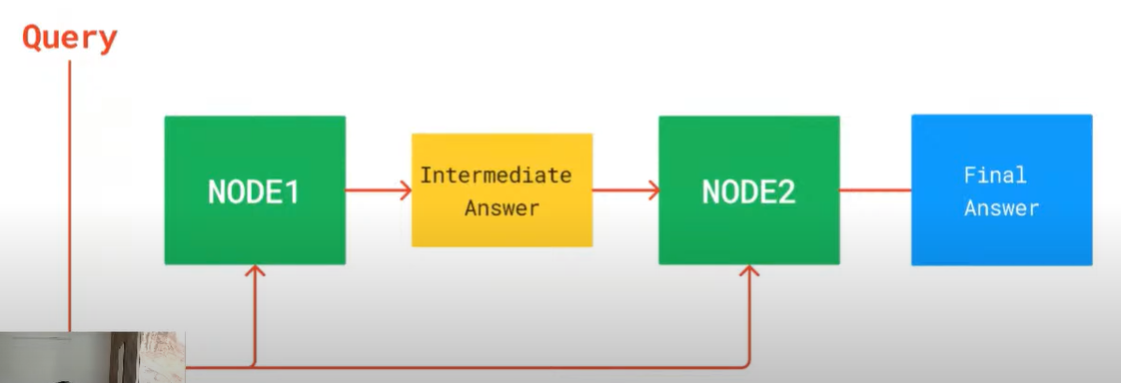
\includegraphics[width=\linewidth,keepaspectratio]{llamaindex14}

% {\tiny (Ref: LlamaIndex: A Central Interface between LLM's + your external data)}
% \end{center}
% \end{frame}


%%%%%%%%%%%%%%%%%%%%%%%%%%%%%%%%%%%%%%%%%%%%%%%%%%%%%%%%%%%
\begin{frame}[fragile]\frametitle{Response Synthesis}

\begin{center}
\includegraphics[width=\linewidth,keepaspectratio]{llm23}

{\tiny (Ref: LlamaIndex: A Central Interface between LLM's + your external data)}
\end{center}
\end{frame}

%%%%%%%%%%%%%%%%%%%%%%%%%%%%%%%%%%%%%%%%%%%%%%%%%%%%%%%%%%%
\begin{frame}[fragile]\frametitle{Response Synthesis}

\begin{center}
\includegraphics[width=0.6\linewidth,keepaspectratio]{llm24}

{\tiny (Ref: LlamaIndex: A Central Interface between LLM's + your external data)}
\end{center}
\end{frame}

%%%%%%%%%%%%%%%%%%%%%%%%%%%%%%%%%%%%%%%%%%%%%%%%%%%%%%%%%%%
\begin{frame}[fragile]\frametitle{Multi level Queries}

\begin{center}
\includegraphics[width=0.6\linewidth,keepaspectratio]{llm25}

{\tiny (Ref: LlamaIndex: A Central Interface between LLM's + your external data)}
\end{center}
\end{frame}

%%%%%%%%%%%%%%%%%%%%%%%%%%%%%%%%%%%%%%%%%%%%%%%%%%%%%%%%%%%
\begin{frame}[fragile]\frametitle{Multi level Queries}

\begin{center}
\includegraphics[width=\linewidth,keepaspectratio]{llm26}

{\tiny (Ref: LlamaIndex: A Central Interface between LLM's + your external data)}
\end{center}
\end{frame}

%%%%%%%%%%%%%%%%%%%%%%%%%%%%%%%%%%%%%%%%%%%%%%%%%%%%%%%%%%%
\begin{frame}[fragile]\frametitle{Multi level Queries}

\begin{center}
\includegraphics[width=\linewidth,keepaspectratio]{llm27}

{\tiny (Ref: LlamaIndex: A Central Interface between LLM's + your external data)}
\end{center}
\end{frame}



%%%%%%%%%%%%%%%%%%%%%%%%%%%%%%%%%%%%%%%%%%%%%%%%%%%%%%%%%%%%%%%%%%%%%%%%%%%%%%%%%%
\begin{frame}[fragile]\frametitle{}
\begin{center}
{\Large Workflows}

{\tiny (Ref: How I Streamline My Research and Presentation with LlamaIndex Workflows - Lingzhen Chen)}
\end{center}
\end{frame}


%%%%%%%%%%%%%%%%%%%%%%%%%%%%%%%%%%%%%%%%%%%%%%%%%%%%%%%%%%%
\begin{frame}[fragile]\frametitle{Introducing LlamaIndex Workflows}
  \begin{itemize}
    \item New feature in LlamaIndex for building flexible, reliable AI pipelines
    \item Allows customized steps with control flow including loops and error handling
    \item Supports cyclical execution, unlike traditional DAG-based pipelines
    \item Ideal for agentic and complex AI workflows
  \end{itemize}
\end{frame}

%%%%%%%%%%%%%%%%%%%%%%%%%%%%%%%%%%%%%%%%%%%%%%%%%%%%%%%%%%%%%%%%%%%%%%%%%%%%%%%%%%
\begin{frame}[fragile]\frametitle{Why Use Workflows for Research Tasks}
  \begin{itemize}
    \item Simplifies research-to-presentation process
    \item Automates paper discovery, summarization, and slide creation
    \item Keeps user in control of intermediate steps and outputs
    \item Enables easy customization and scaling
  \end{itemize}
\end{frame}

%%%%%%%%%%%%%%%%%%%%%%%%%%%%%%%%%%%%%%%%%%%%%%%%%%%%%%%%%%%%%%%%%%%%%%%%%%%%%%%%%%
\begin{frame}[fragile]\frametitle{Motivation for a Custom Workflow}
  \begin{itemize}
    \item Maintain an existing research process while improving efficiency
    \item Centralized end-to-end solution for summarization and slide generation
    \item Retain control over intermediate outputs for fine-tuning
    \item Future-proof with extensibility and modularity
  \end{itemize}
\end{frame}

%%%%%%%%%%%%%%%%%%%%%%%%%%%%%%%%%%%%%%%%%%%%%%%%%%%%%%%%%%%%%%%%%%%%%%%%%%%%%%%%%%
\begin{frame}[fragile]\frametitle{Workflow Example: Research to Presentation}
  \begin{itemize}
    \item User provides a research topic (e.g., “GenAI for slides”)
    \item Pulls relevant papers from arXiv.org
    \item Summarizes each paper using LLMs
    \item Extracts key insights: approach, model, dataset, evaluation, results
    \item Outputs one slide per paper with structured summaries
  \end{itemize}
\end{frame}

%%%%%%%%%%%%%%%%%%%%%%%%%%%%%%%%%%%%%%%%%%%%%%%%%%%%%%%%%%%%%%%%%%%%%%%%%%%%%%%%%%
\begin{frame}[fragile]\frametitle{Core Concepts: Steps and Events}
  \begin{itemize}
    \item \textbf{Step}: Python function for discrete tasks in the workflow
    \item Steps can share context and communicate using events
    \item \textbf{Event}: Pydantic objects that control data flow and execution
    \item Special events include StartEvent and StopEvent
  \end{itemize}
\end{frame}

%%%%%%%%%%%%%%%%%%%%%%%%%%%%%%%%%%%%%%%%%%%%%%%%%%%%%%%%%%%%%%%%%%%%%%%%%%%%%%%%%%
\begin{frame}[fragile]\frametitle{Advanced Workflow Features}
  \begin{itemize}
    \item Async and parallel execution to boost performance
    \item Nested workflows for hierarchical structure
    \item Structured LLM output ensures clean data flow
    \item Dynamic session supports isolated code execution
    \item Use of specialized agents for different steps
    \item Varying LLM models (e.g., gpt-4o, gpt-4o-mini) for optimized tasks
  \end{itemize}
\end{frame}

%%%%%%%%%%%%%%%%%%%%%%%%%%%%%%%%%%%%%%%%%%%%%%%%%%%%%%%%%%%%%%%%%%%%%%%%%%%%%%%%%%
\begin{frame}[fragile]\frametitle{Getting Started and Resources}
  \begin{itemize}
    \item Requires API keys for Tavily, Semantic Scholar, and Azure OpenAI
    \item Full implementation available on GitHub
    \item Compatible with OpenAI or other models via LlamaIndex
    \item Additional support via notebooks and video tutorials
  \end{itemize}
\end{frame}

%%%%%%%%%%%%%%%%%%%%%%%%%%%%%%%%%%%%%%%%%%%%%%%%%%%%%%%%%%%
\begin{frame}[fragile]\frametitle{Main Workflow Structure}
  \begin{itemize}
    \item Consists of two nested sub-workflows: \texttt{summary\_gen} and \texttt{slide\_gen}
    \item \textbf{summary\_gen}: Searches for research papers and uses LLMs to generate topic-specific summaries
    \item \textbf{slide\_gen}: Converts summaries into PowerPoint slides using a template and \texttt{python-pptx}
    \item Executes and formats slides via dynamic Python code generation
  \end{itemize}
\end{frame}


%%%%%%%%%%%%%%%%%%%%%%%%%%%%%%%%%%%%%%%%%%%%%%%%%%%%%%%%%%%
\begin{frame}[fragile]\frametitle{The Main workflow}

\begin{center}
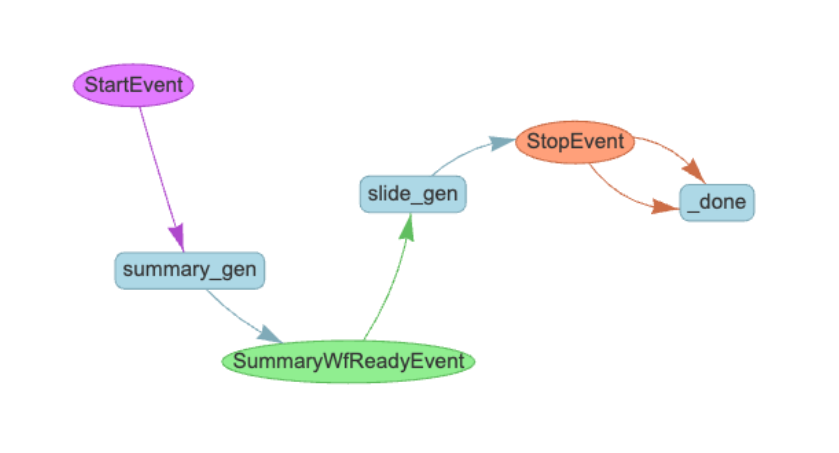
\includegraphics[width=\linewidth,keepaspectratio]{llamaindex22}

{\tiny (Ref: How I Streamline My Research and Presentation with LlamaIndex Workflows - Lingzhen Chen)}
\end{center}
\end{frame}

%%%%%%%%%%%%%%%%%%%%%%%%%%%%%%%%%%%%%%%%%%%%%%%%%%%%%%%%%%%
\begin{frame}[fragile]\frametitle{Summary Generation Sub-workflow}
  \begin{itemize}
    \item \texttt{summary\_gen} is a linear, data-processing workflow
    \item Executes a series of steps to find and summarize research papers
    \item Some steps interact with an LLM to extract insights
    \item Designed for simplicity and clarity in processing academic content
    \item Starts with user-provided research topic
    \item \texttt{tavily\_query}: Uses Tavily API to fetch relevant academic papers
    \item \texttt{get\_paper\_with\_citations}: Retrieves metadata for each paper and its citations via SemanticScholar API
    \item \texttt{filter\_papers}: Uses LLM to evaluate and filter papers based on relevance
    \item \texttt{filter\_papers} step runs in parallel with \texttt{@step(num\_workers=4)} for efficiency	
  \end{itemize}
\end{frame}


%%%%%%%%%%%%%%%%%%%%%%%%%%%%%%%%%%%%%%%%%%%%%%%%%%%%%%%%%%%
\begin{frame}[fragile]\frametitle{Summary Generation Sub-workflow}

\begin{center}
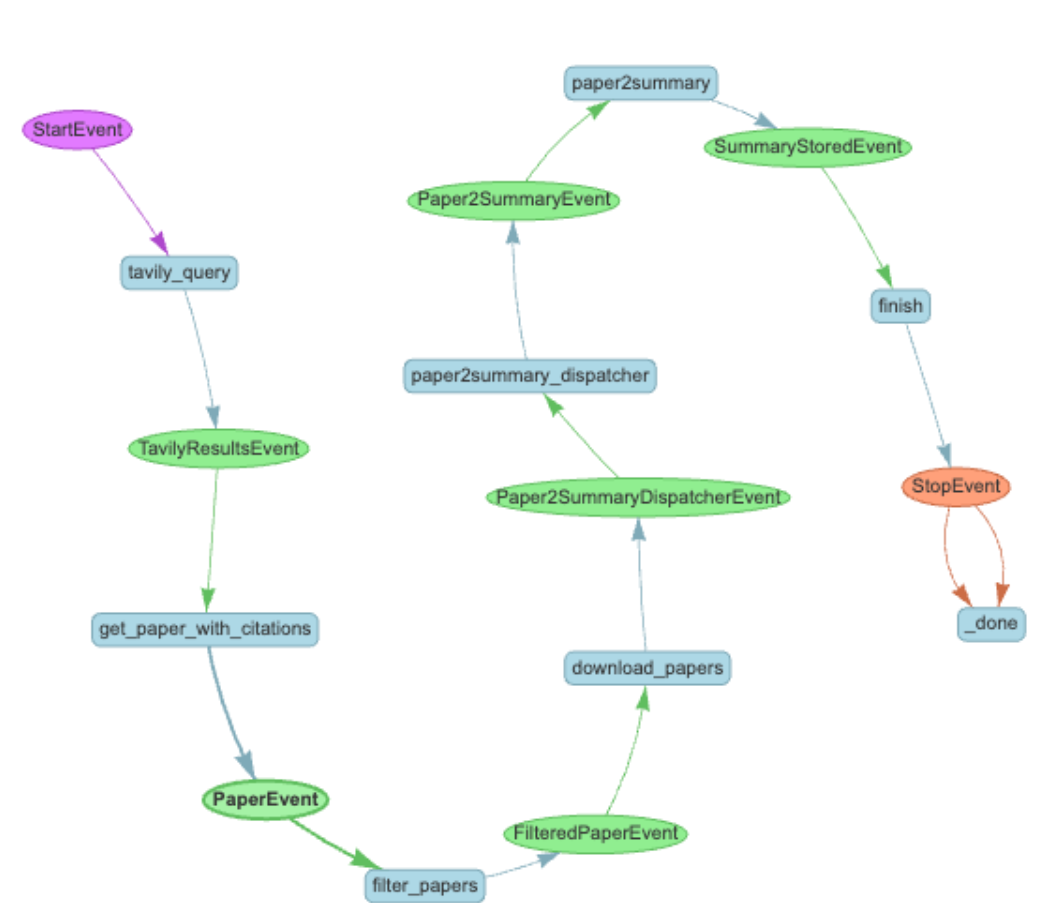
\includegraphics[width=0.7\linewidth,keepaspectratio]{llamaindex23}

{\tiny (Ref: How I Streamline My Research and Presentation with LlamaIndex Workflows - Lingzhen Chen)}
\end{center}
\end{frame}

%%%%%%%%%%%%%%%%%%%%%%%%%%%%%%%%%%%%%%%%%%%%%%%%%%%%%%%%%%%
\begin{frame}[fragile]\frametitle{Additional Steps in Summary Generation}
  \begin{itemize}
    \item \texttt{download\_papers}: Prioritizes and downloads the most relevant papers based on ArXiv availability and relevance score
    \item \texttt{paper2summary\_dispatcher}: Prepares papers for summarization, enabling parallel execution of \texttt{paper2summary}
    \item \texttt{paper2summary}: Converts PDFs to images, sends them to LLM for detailed summaries, saves in markdown for future reference
    \item \texttt{finish}: Verifies summary storage, logs completion, and triggers the next sub-workflow \texttt{slide\_gen}
  \end{itemize}
\end{frame}

%%%%%%%%%%%%%%%%%%%%%%%%%%%%%%%%%%%%%%%%%%%%%%%%%%%%%%%%%%%
\begin{frame}[fragile]\frametitle{The Slide Generation Sub-workflow}

\begin{center}
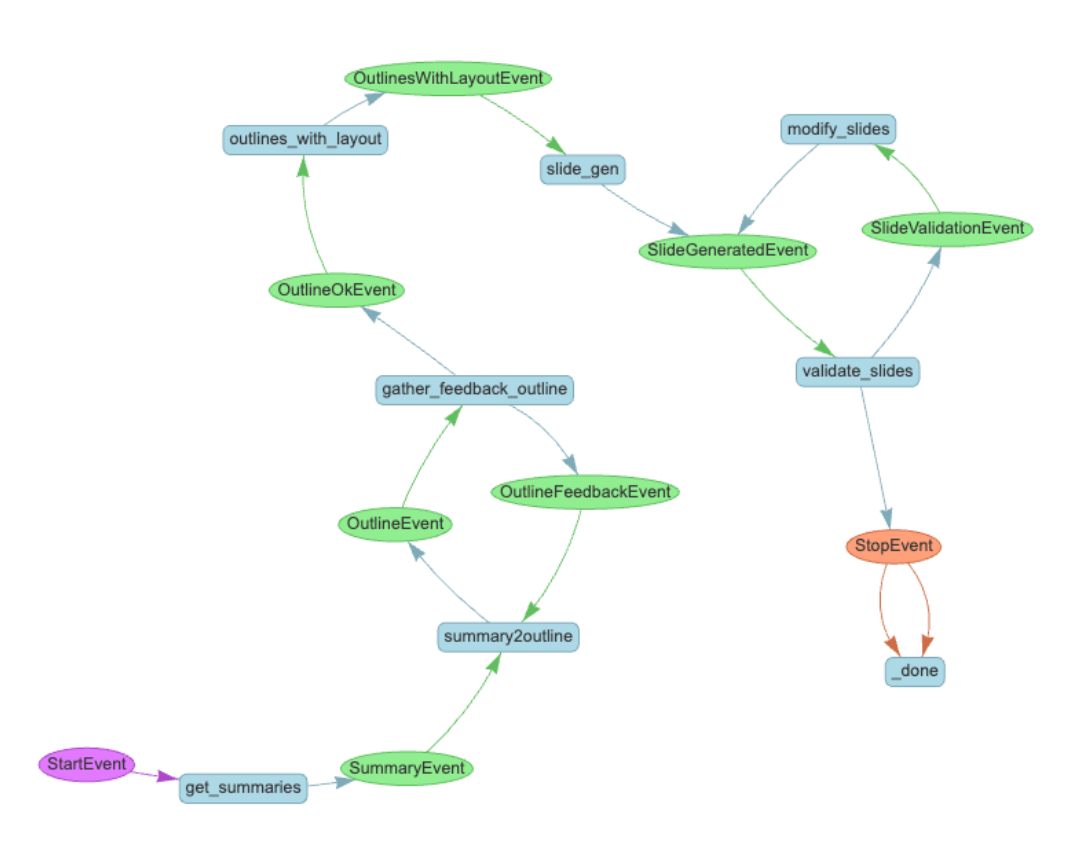
\includegraphics[width=0.8\linewidth,keepaspectratio]{llamaindex24}

{\tiny (Ref: How I Streamline My Research and Presentation with LlamaIndex Workflows - Lingzhen Chen)}
\end{center}
\end{frame}

%%%%%%%%%%%%%%%%%%%%%%%%%%%%%%%%%%%%%%%%%%%%%%%%%%%%%%%%%%%
\begin{frame}[fragile]\frametitle{Slide Generation Sub-workflow}
  \begin{itemize}
    \item Starts after summary markdown files are ready from \texttt{summary\_gen}
    \item \texttt{get\_summaries}: Reads summary files and triggers concurrent execution via \texttt{SummaryEvent}
    \item \texttt{summary2outline}: Converts summaries into concise slide outlines using LLM
    \item \texttt{gather\_feedback\_outline}: Presents outline to user for feedback; loop continues until approval
    \item \texttt{outlines\_with\_layout}: Enhances slide outlines with layout details from PowerPoint template
    \item \texttt{slide\_gen}: Uses ReAct agent with \texttt{python-pptx} to generate slides
    \item \texttt{validate\_slides}: LLM visually inspects slides for content and style, sends \texttt{SlideValidationEvent} if errors are found
    \item \texttt{modify\_slides}: If validation fails, ReAct agent updates slides based on feedback and re-validates
  \end{itemize}
\end{frame}

%%%%%%%%%%%%%%%%%%%%%%%%%%%%%%%%%%%%%%%%%%%%%%%%%%%%%%%%%%%
\begin{frame}[fragile]\frametitle{Final Thoughts and Observations}
  \begin{itemize}
    \item \textbf{GPT-4o vs GPT-4o-mini}: GPT-4o-mini struggles with complex tasks but performs well in simpler ones (e.g., summarizing)
    \item \textbf{Intermediate files}: Useful for easing agent workload and ensuring content and style consistency
    \item \textbf{Handling edge cases}: Iterative prompts address style validation issues; human-in-the-loop could improve accuracy
    \item \textbf{python-pptx limitations}: Consider alternatives like VBA for more efficient slide generation
    \item \textbf{Agents and tools}: Agents with tool access can offer flexibility and adaptability for future changes
    \item \textbf{Enhance human interaction}: More user involvement in validation and refinement would improve results
    \item \textbf{Personalized query engines}: Allow users to query papers and modify summaries for tailored results
    \item \textbf{LlamaIndex flexibility}: A powerful tool for building customizable AI solutions with both control and flexibility
  \end{itemize}
\end{frame}

